\documentclass[10pt,a4paper]{article}
\usepackage[utf8]{inputenc}
\usepackage[T1]{fontenc}
\usepackage[english]{babel}
\usepackage{amsmath}
\usepackage{amsfonts}
\usepackage{amssymb}
\usepackage{graphicx}

\author{Jakub Kocalka, xkocal00}
\title{Accidents with Trailers}
\begin{document}
	\maketitle
	
	This article will explore the effect of trailers on accidents involving personal vehicles.
	
	\begin{table}[h]
		\centering
		\begin{tabular}{p{27mm}|cc|}
			Serious Accident \newline Trailer & False & True \\
			\hline 
			False & 297197 & 7230 \\ 
			True & 2673 & 86 \\ 
		\end{tabular}
		\caption{Accident seriousness vs trailer use}
		\label{tab:cross}
	\end{table}

	Table 1 is a contingency table describing the relationship between accident seriousness (serious accident is an accident that resulted in loss of life or a serious injury) and trailer use.
	
	\begin{table}[h]
		\centering
		\begin{tabular}{c|c}
			$\chi^2$ statistic & 6.161748797182163\\
			p-value & 0.013054208299270505\\
		\end{tabular}
		\caption{Results of the $\chi^2$ test}
		\label{tab:chi_result}
	\end{table}
	
	Using the $\chi$-squared test, we conclude, that accident seriousness and trailer use are related, in particular, the presence of a trailer in an accident makes it more likely to be serious.
	
	Next, let's explore the causes of accidents involving trailers.
	
	\begin{figure}
		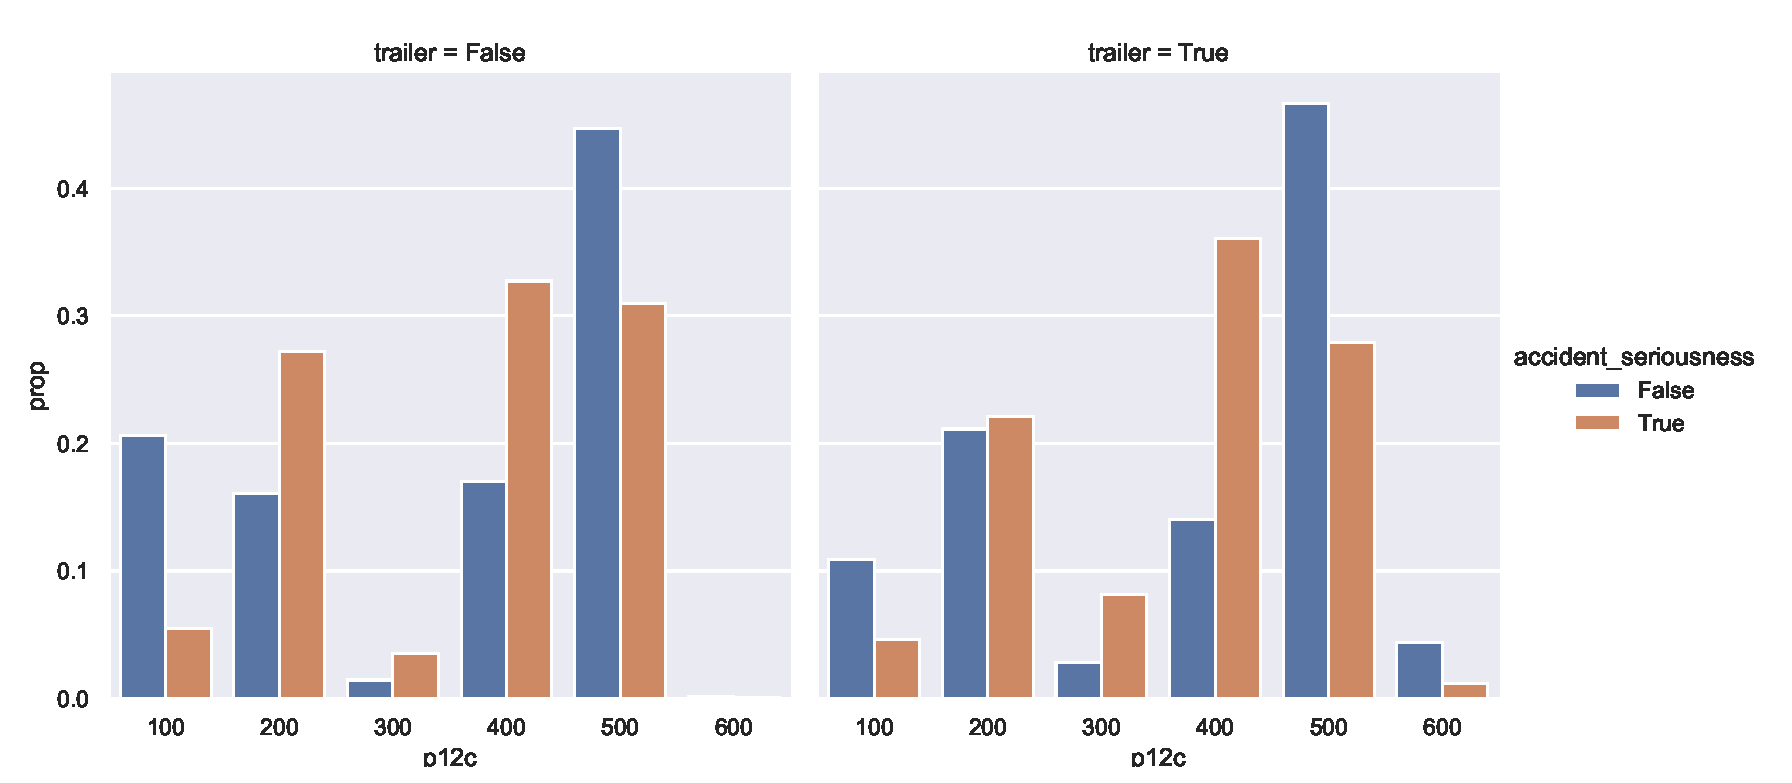
\includegraphics[width=\textwidth]{fig.eps}
		\caption{Accident Causes}
		\label{fig:causes}
	\end{figure}
	 
	
\end{document}